\section{决策部分}
\label{sec:policy}
\begin{frame}{决策部分}
    \begin{itemize}
        \item 输入:语义地图 (semantic map)
        \item 输出:
            \begin{itemize}
                \item 长期目标 (long-term goal)
                \item 当前行动 (action, path)
                \begin{itemize}
                    \item $a_t$: 向前,左转,右转,停
                \end{itemize}
            \end{itemize}
    \end{itemize}
    \note{
        \begin{itemize}
            \item 决策部分负责接受感知部分输出的语义地图,并分成两步完成决策
            \item 第一步全局决策:选择一个long-term goal,表示在未来的一段时间内目标到达的位置
            \item 第二步局部决策:决定为了到达long-term goal,应该如何行动
        \end{itemize}
    }
\end{frame}


\begin{frame}{决策部分总体结构}
    \centering
    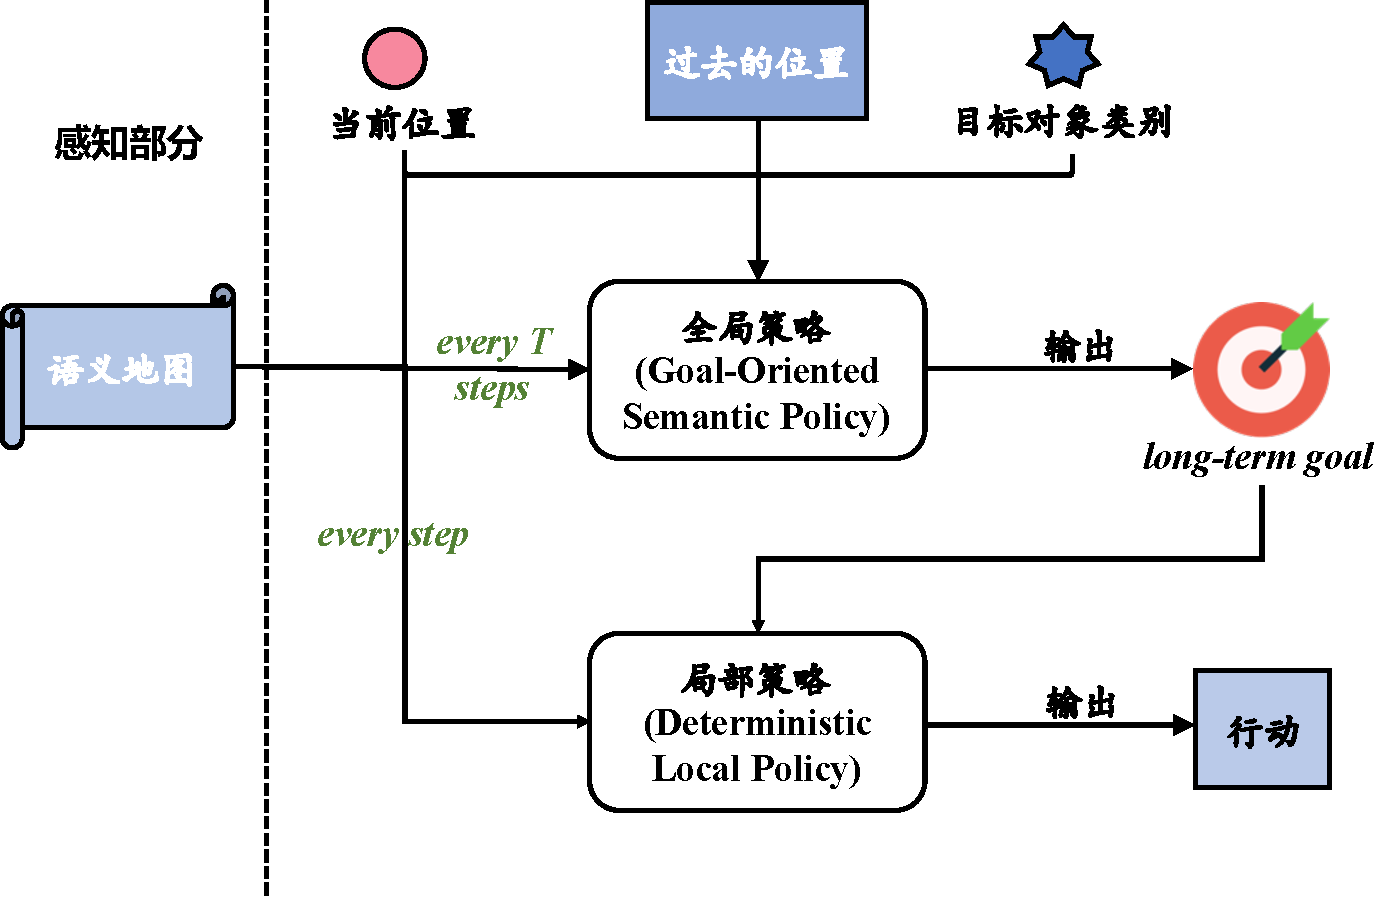
\includegraphics[width=11cm]{assets/policy_structure.pdf}
    \note{
        决策部分可以大致分为两个部分:全局决策和局部决策
        \begin{itemize}
            \item 全局决策:得到长期目标 (\emph{long-term goal})
                \begin{itemize}
                    \item 输入:语义地图,当前位置,过去的位置,目标对象的类别
                    \item coarse time scale: 每25步更新一次long-term goal(减少复杂度)
                    \item 采用强化学习的方式进行训练~\cite{...}
                \end{itemize}
            \item 局部决策:得到抵达long-term goal的路径 (path)
                \begin{itemize}
                    \item 输入:语义地图,当前位置,long-term goal
                    \item 也就知道了当前应该采取的行动$a_t$
                    \item fine time scale: 每一步都需要决策
                    \item 采用Far Marching Method~\cite{...}
                \end{itemize}
        \end{itemize}
    }
\end{frame}

\begin{frame}{全局决策}
    采用的策略: Goal-Oriented Semantic Policy
\end{frame}

\begin{frame}{局部决策}
    采用的方法: Far Marching Method
\end{frame}